%\documentclass[useAMS, usenatbib,usegraphicx,letter]{mn2e}
%\documentclass[11pt]{article}
\documentclass[reprint,aps,prd,superscriptaddress,showkeys,showpacs]{revtex4-1}
\usepackage{epsfig,amsmath,natbib}

\usepackage{aas_macros}
\usepackage{amssymb}
\usepackage{amsmath}
\usepackage{dsfont}
\usepackage{hyperref}
\usepackage{color}
\usepackage{pbox}
\usepackage{booktabs}

\hypersetup{
	colorlinks=false,
	citecolor=green
}
% \usepackage{graphicx}
% \usepackage{epstopdf}
% \usepackage{natbib}

%%%%%%%%%%%%%%%%%
%Custom commands%
%%%%%%%%%%%%%%%%%

\newcommand{\bb}[1]{\mathbf{#1}}
\newcommand{\bbh}[1]{\mathbf{\hat{#1}}}
\newcommand{\h}[1]{\hat{#1}}

%%%%%%%%%%%%%%%%%%%%%%%%%%%%%%%%%%%%%%%%%%%%%%

\begin{document}

\title{Simulating cosmic variance in Weak Lensing: effects on parameter inferences}

\author{Andrea Petri}
\email{apetri@phys.columbia.edu}
\affiliation{Department of Physics, Columbia University, New York, NY 10027, USA}
\affiliation{Physics Department, Brookhaven National Laboratory, Upton, NY 11973, USA}

\author{Zolt\'an Haiman}
\affiliation{Department of Astronomy, Columbia University, New York, NY 10027, USA}

\author{Morgan May}
\affiliation{Physics Department, Brookhaven National Laboratory, Upton, NY 11973, USA}

\date{\today}

\label{firstpage}

\begin{abstract}
Constraining cosmology using Weak Gravitational Lensing consists in comparing measured features with simulated ones. An accurate estimate of the feature covariance matrix is essential to obtain accurate parameter confidence intervals. When this covariance matrix $\bb{C}$ is measured from simulations, an important question to ask is how big the simulation set should be for an accurate estimation of $\bb{C}$. We construct different mock ensembles with $N_r$ realizations of the same shear field, based on $N_s<N_r$ independent $N$--body simulations. Using the shear--shear power spectrum as a summary statistic, we find that the scaling of the forecasted error bar for $w$ shows the expected behavior with $N_r$ (see \citep{DodelsonSchneider13}). The same quantity shows a mild dependence on $N_s$ and on the effective dimensionality of the feature space.     
\end{abstract}


\keywords{Weak Gravitational Lensing --- Simulations --- Methods: numerical,statistical}
\pacs{98.80.-k, 95.36.+x, 95.30.Sf, 98.62.Sb}

\maketitle


%%%%%%%%%%%%%%%%%%%%%%%%%% INTRO %%%%%%%%%%%%%%%%%%%%%%%%%%%%%%%%%%%%%%%%%%%%%%%%%%%%%%%%

\section{Introduction}
%
Weak Gravitational lensing is a promising cosmological probe for constraining the Dark Energy equation of state $w$, and has been considered by a range of past (CFHTLens \citep{cfht1,cfht2}), current (DES \citep{DES}) and future (LSST \citep{LSST}) experiments. In an era where cosmology is becoming data driven, accurate numerical simulations of shear fields are becoming important for a number of reasons including the study of baryonic effects \citep{BaryonXiuyuan}, non--Gaussian statistics \citep{PeaksJan,MinkJan,MinkPetri} and various systematics. Building cosmological predictions from simulations naturally introduces fluctuations in the forecasts, mainly due to cosmic variance. These fluctuations have been shown to have non negligible effects on estimates of features covariance matrices and hence on parameter constraints (see \citep{DodelsonSchneider13}). This work studies this issue further, focusing on the number of independent $N$--body simulations that is necessary to run for obtaining accurate estimates of parameter constraints, with particular focus on $w$. This paper is organized as follows: in the first paragraph we briefly describe the shear simulation methods we used, as well as the formalism we adopted to compute cosmological parameter constraints. We then outline our main findings and discuss the results, as well as future prospects for continuing this study.  

%%%%%%%%%%%%%%%%%%% METHODS %%%%%%%%%%%%%%%%%%%%%%%%%%%%%%%%%%%%%%%

\section{Methods}

\subsection{Shear field simulations}
\label{shearsim}
%
In this paragraph we describe how we constructed our shear field ensembles. Background galaxies at redshift $z_s$ are lensed by large scale structure between $z=0$ and $z_s$. The shape distortions due to the cosmic shear $\pmb{\gamma}$ can be computed in terms of the dark matter gravitational potential $\Phi(\bb{x},z)$. Because the evolution of $\Phi$ in redshift is non--linear, its evolution needs to be computed with numerical simulations. We make use of the public code Gadget2 \citep{Gadget2}, with which we run a sequence of dark--matter--only $N$--body simulations that track the evolution of the density fluctuations in the large scale structure of the universe. We assume a standard $\Lambda$CDM framework with $(\Omega_m,\Omega_\Lambda,h,w,\sigma_8,n_s)=(0.26,0.74,0.72,-1,0.8,0.96)$ and we fix the comoving size of the simulation box to $240\mathrm{Mpc}/h$. We fill the box with $512^3$ particles, which correspond to a mass resolution of $10^{10}M_\odot$. We assume a uniform galaxy distribution at a constant redshift $z_s=2$ (at which the simulation box has an angular size of $\theta_{box}=3.5\mathrm{deg}$) and we disctretize the mass distribution between $z_s$ and the observer at $z=0$ with a sequence of 60 two dimensional lenses of thickness $80\mathrm{Mpc}/h$. The surface density on each lens is computed by projecting the three dimensional density measured from Gadget2 snapshots. We then apply the multi--lens--plane algorithm (see \citep{RayTracingHartlap,RayTracingJain} for example) to trace the deflections of $2048^2$ light rays arranged on a square grid of total size $\theta_{box}$, from $z=0$ to $z_s$. The light deflection calculations have been performed with our implementation of multi--lens--plane algorithm, which is part of the LensTools computing package \citep{LensTools} (released under the MIT license). Different realizations $r$ of the same shear field $\pmb{\gamma}_r(\pmb{\theta})$ can be generated with different choices of the lenses that lay between the observer and $z_s$. The randomization procedure we adopt is the following:

\begin{itemize}
\item Pick a lens redshift $z_l$, and select the snapshot at $z_l$ from the $i$--th $N$--body simulation at disposal, where $i$ is a random number in $[1,N_s]$
\item Choose randomly a direction in $(\bb{n}_x,\bb{n}_y,\bb{n}_z)$: the lens plane will be pependicular to this direction
\item Choose the cutting point of the plane in the snapshot: because the lenses are $80\mathrm{Mpc}/h=240/3\mathrm{Mpc}/h$ thick, we have 3 different possibilities for choosing the random cut point
\item Perform a periodical random shift of the lens plane along its two directions
\item Repeat this procedure for each lens redshift $z_l$  
\end{itemize}  
%
This randomization procedure allows us to produce an arbitrary number $N_r$ of mock shear realizations $\pmb{\gamma}_r(\pmb{\theta})$, which however will not be all independent if $N_s$ is not large enough. Using a set of 200 independent $N$--body simulations, we construct different ensembles with different choices of $N_s\in[1,200]$, each made of 1000 mock shear realizations. From each of these mocks we reconstruct the convergence $\kappa_r(\pmb{\theta})$ and measure its angular power spectrum $P^{\kappa\kappa}_r(l)$ defined as
\begin{equation}
\langle\tilde{\kappa}_r(\bb{l})\tilde{\kappa}_r(\bb{l}')\rangle = (2\pi)^2\delta_D(\bb{l}+\bb{l}')P^{\kappa\kappa}_r(l)
\end{equation}
%
The fact that the ensemble of $N_r$ mocks is not completely independent if $N_s$ is not large enough can have an effect on the covariance estimator of $P^{\kappa\kappa}$. 

\subsection{Parameter inference}
%
Let $\bbh{d}$ be the measured feature of dimension $N_b$, $\bb{d}(\bb{p})$ be the simulated feature at a point $\bb{p}$ in parameter space and $\bb{C}$ be the $N_b\times N_b$ feature covariance matrix. For the purpose of this work $\bb{p}$ is the triplet $(\Omega_m,w,\sigma_8)$ and $\bb{d}$ is the convergence power spectrum $P^{\kappa\kappa}$, which is measured at $N_b=15$ log--spaced bands between $l\in[100,6000]$. While $d_M(\bb{p})$ can usually be predicted reasonably accurately by already existing emulators (see \citep{coyote2,Nicaea} for example), the matter is more complicated for covariance matrices. Measuring $\bb{C}$ from simulations involves generating a series of mock realizations $\bbh{d}_r$ with $r=1...N_r$ and estimating the sample covariance $\bbh{C}$

\begin{equation}
\bb{\bar{d}} = \frac{1}{N_r}\sum_{r=1}^{N_r} \bbh{d}_r
\end{equation}

\begin{equation}
\label{covest}
\bbh{C} = \frac{1}{N_r-1}\sum_{r=1}^{N_r} (\bbh{d}_r - \bar{\bb{d}}) (\bbh{d}_r - \bar{\bb{d}})^T
\end{equation}
%
Assuming a normal feature likelihood, together with a flat prior on the parameter space, the parameter posterior distribution $\mathcal{L}(\bb{p}\vert\bbh{d})$ can be obtained using Bayes theorem
\begin{equation}
\label{posteriorbayes}
\mathcal{L}(\bb{p}\vert\bbh{d}) = \mathcal{N}_\mathcal{L}\exp{\left[-\frac{1}{2}(\bbh{d}-\bb{d}(\bb{p}))^T\bb{C}^{-1}(\bbh{d}-\bb{d}(\bb{p}))\right]}
\end{equation}
%
For the sake of simplicity, we approximate the posterior as a Gaussian around its maximum. This is easily done approximating the simulated feature at first order around a point $\bb{p}_0$ (that ideally is the maximum of (\ref{posteriorbayes}))
\begin{equation}
\bb{d}(\bb{p}) \approx \bb{d}_0 + \bb{d}_0^\prime(\bb{p}-\bb{p}_0) 
\end{equation}
%
From which we can build the estimators for the parameters expectation value $\bbh{p}$ and covariance $\h{\Sigma}_\bb{p}$, given the observation $\bbh{d}$, as follows:
%
\begin{equation}
\label{estimatormean}
\bbh{p} = \bb{p}_0 + \bbh{T}(\bbh{d}-\bb{d}_0)
\end{equation}

\begin{equation}
\label{estimatorcovariance}
\h{\Sigma}_\bb{p} = \bbh{T}(\bbh{d}-\bb{d}_0)(\bbh{d}-\bb{d}_0)^T\bbh{T}^T
\end{equation}

\begin{equation}
\bbh{T} = (\bb{d}_0'^T\bbh{C}^{-1}\bb{d}_0')^{-1}\bb{d}_0'^T\bbh{C}^{-1}
\end{equation}
%
Where, for simplicity we assumed $\langle\bbh{d}\rangle=\bb{d}_0$, so that $\langle(\bbh{d}-\bb{d}_0)(\bbh{d}-\bb{d}_0)^T\rangle=\bb{C}$. Since the feature we consider is the shear-shear power spectrum, its derivatives $\bb{d}_0'$ with respect to the cosmological parameters can be evaluated by existing analytical codes. For this purpose we use the analytical code NICAEA (see \citep{Nicaea}). The noise in the covariance estimator (\ref{covest}) propagates all the way to the posterior (\ref{posteriorbayes}), the parameter estimate (\ref{estimatormean}) and its variance (\ref{estimatorcovariance}), through the transformation matrix $\bbh{T}$. \citep{DodelsonSchneider13} found that the variance $\h{\sigma}^2_\bb{p}=\mathrm{diag}(\bbh{\Sigma}_\bb{p})$ of each parameter $p$ that is estimated from (\ref{estimatorcovariance}) increases on average with $1/N_r$
\begin{equation}
\label{dodelsonscaling}
\langle\h{\sigma}_\bb{p}^2\rangle = \sigma_p^2\left(1+\frac{D}{N_r}\right)
\end{equation} 
%
where $\sigma^2_p$ is the true parameter variance and $D$ is what we call \textit{effective dimensionality} of the feature space. \citep{DodelsonSchneider13} found $D=N_b$ when every entry in the covariance matrix is subject to noise. In this work we argue that the feature ensemble from which the covariance estimator $\bbh{C}^{-1}$ is measured depends not only on the number of shear mock realizations $N_r$, but in principle also on the number of independent $N$--body simulations $N_s$, on which the randomization procedure we describe in \S~\ref{shearsim}. We propose a modification to the scaling relation (\ref{dodelsonscaling}) that takes the varying $N_s$ into account. 

\begin{equation}
\label{ourscaling}
\langle\h{\sigma}_p^2\rangle = \sigma^2_p(N_s,D)\left(1+\frac{D}{N_r}\right)
\end{equation} 
%
The reason for this can be found in that, if $N_s$ is not big enough, the different shear realizations cannot be all independent, and hence the true variance $\sigma^2_p$ cannot be recovered in the limit $N_r\rightarrow\infty$. In particular there could be some residual error in the expectation value of (\ref{estimatorcovariance}) even if $N_r$ is big. In the next paragraph we outline our main findings. 

%%%%%%%%%%%%%%%%%%% RESULTS %%%%%%%%%%%%%%%%%%%%%%%%%%%%%%%%%%%%%%%

\section{Results}

\begin{figure*}
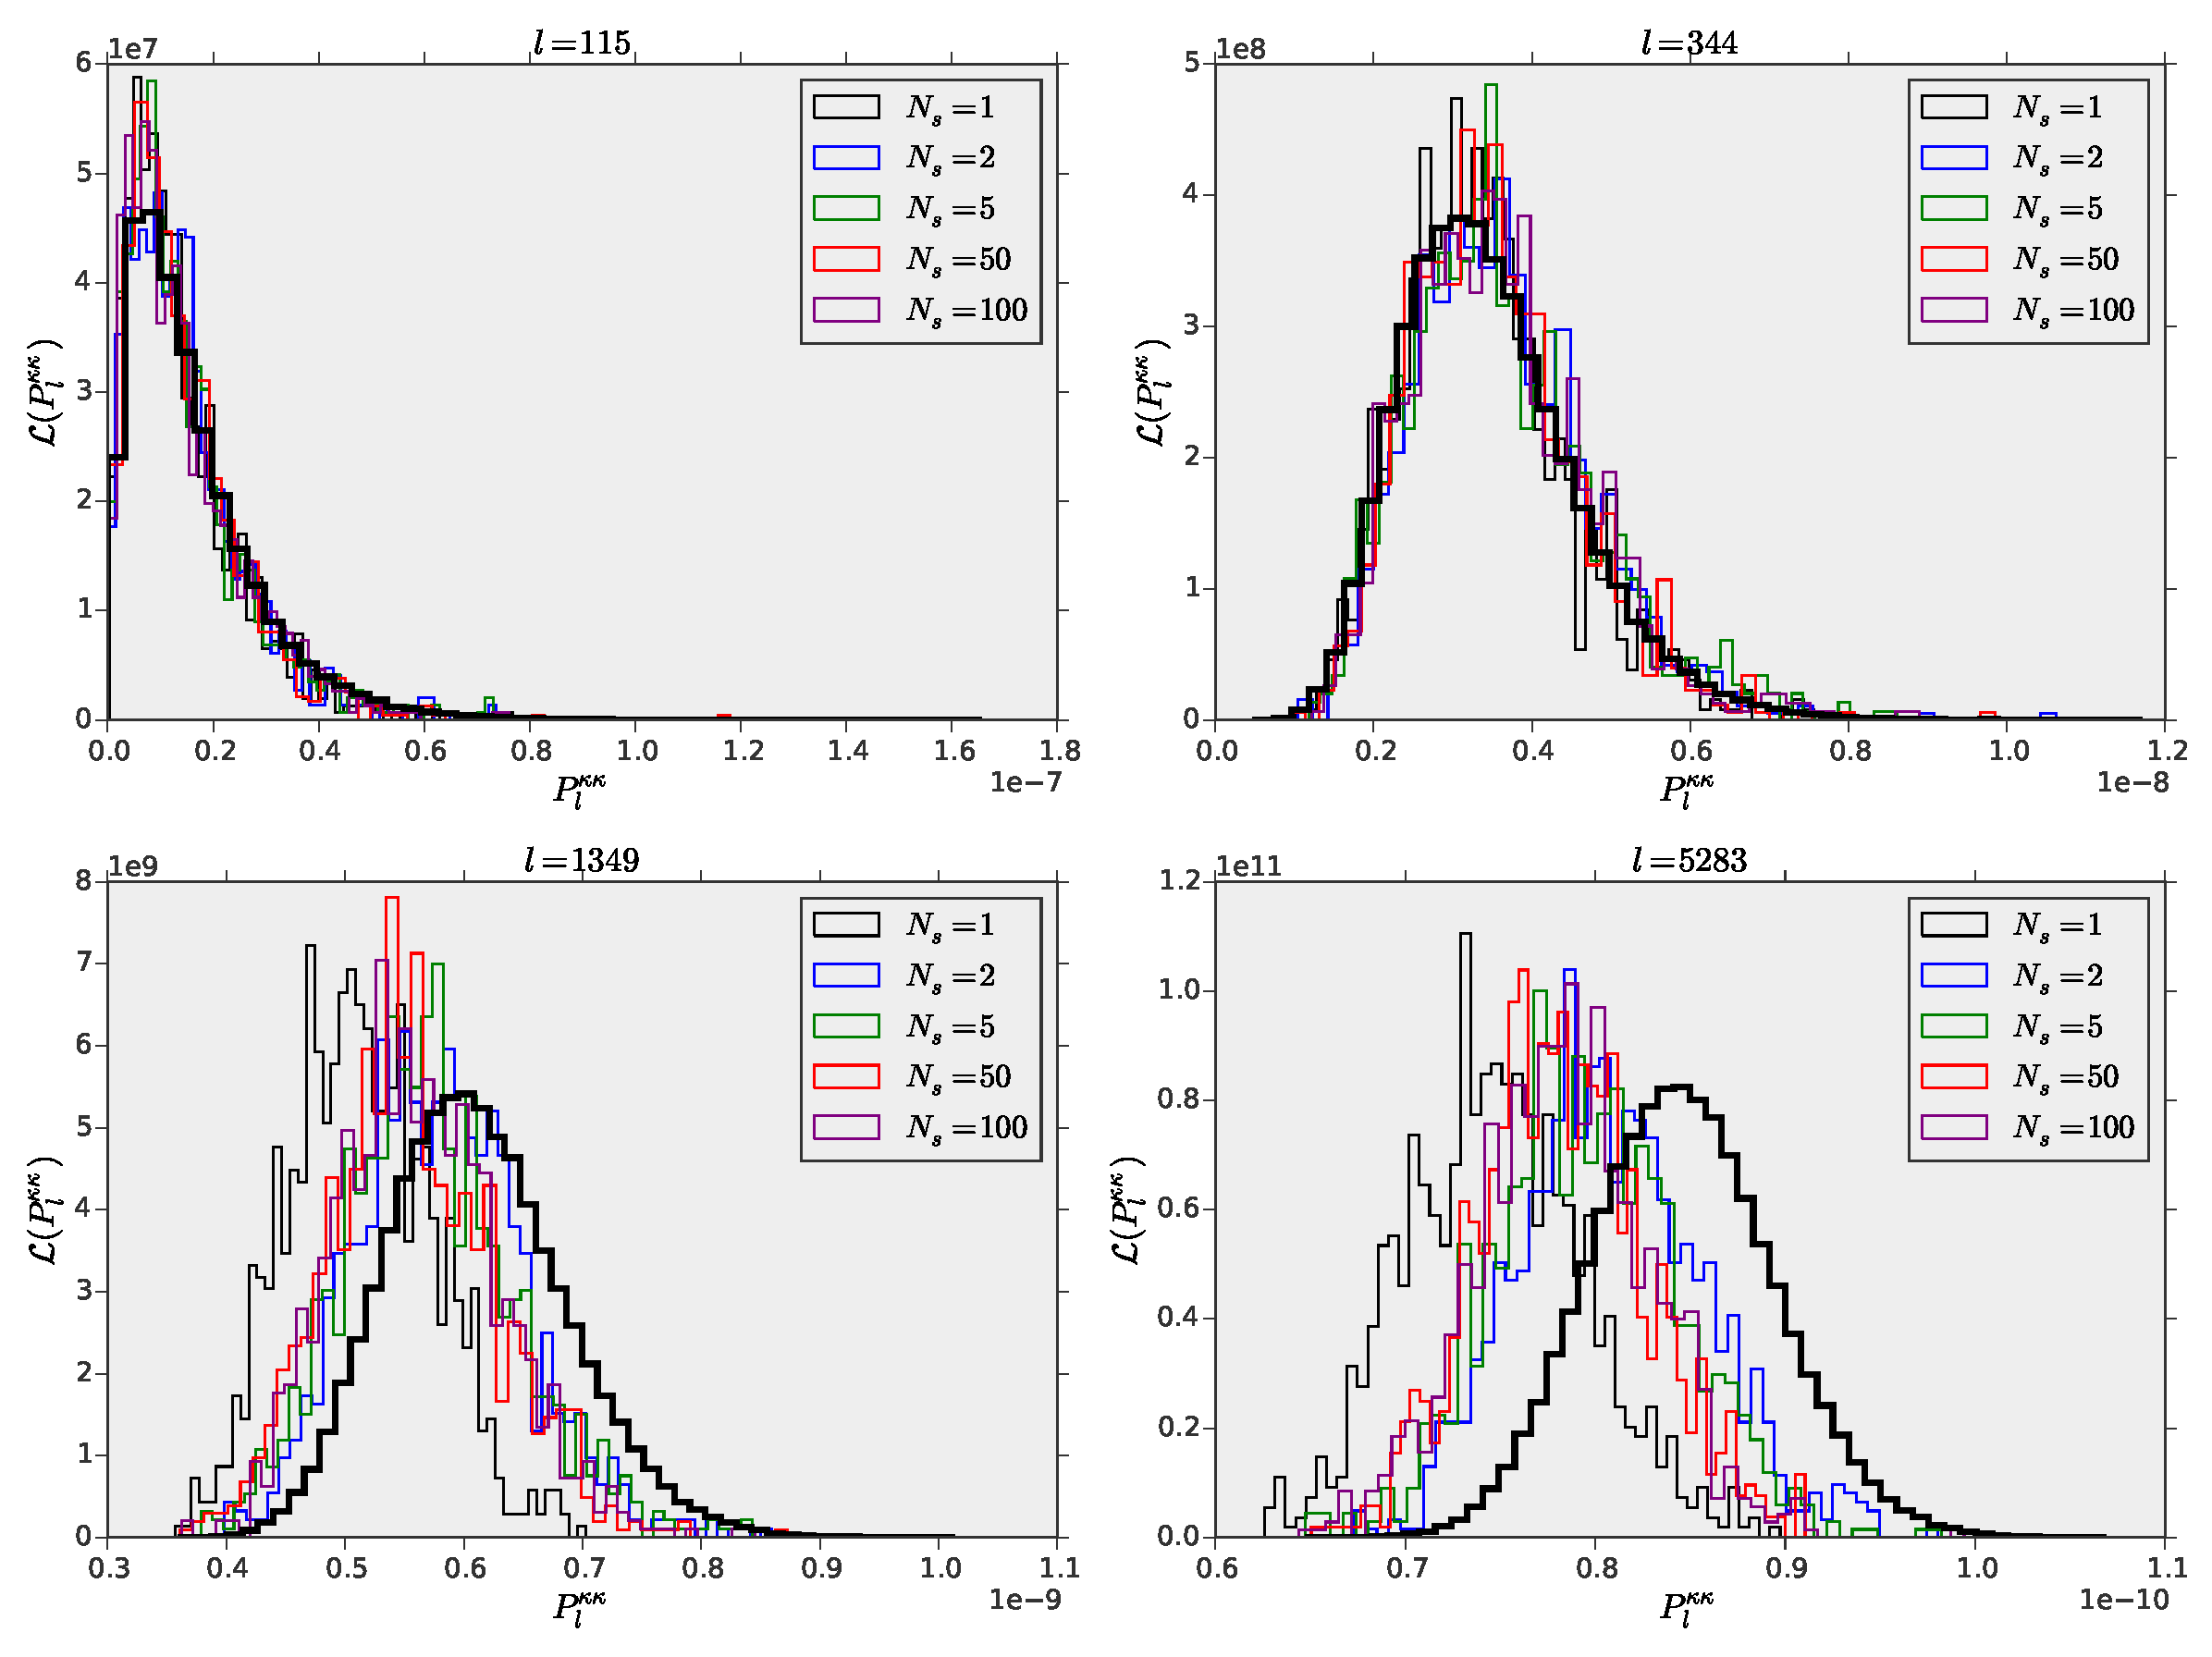
\includegraphics[scale=0.4]{Figures/ps_pdf.eps}
\caption{PDF of the $\kappa$ power spectrum,$\mathcal{L}(P_l^{\kappa\kappa})$, at four selected multipoles $l=115,344,1349,5283$, for different shear ensembles constructed with $N_s=$1 (black), 2 (blue), 5 (green), 50 (red), 100 (purple).}
\label{ps_pdf}
\end{figure*}

\begin{figure}
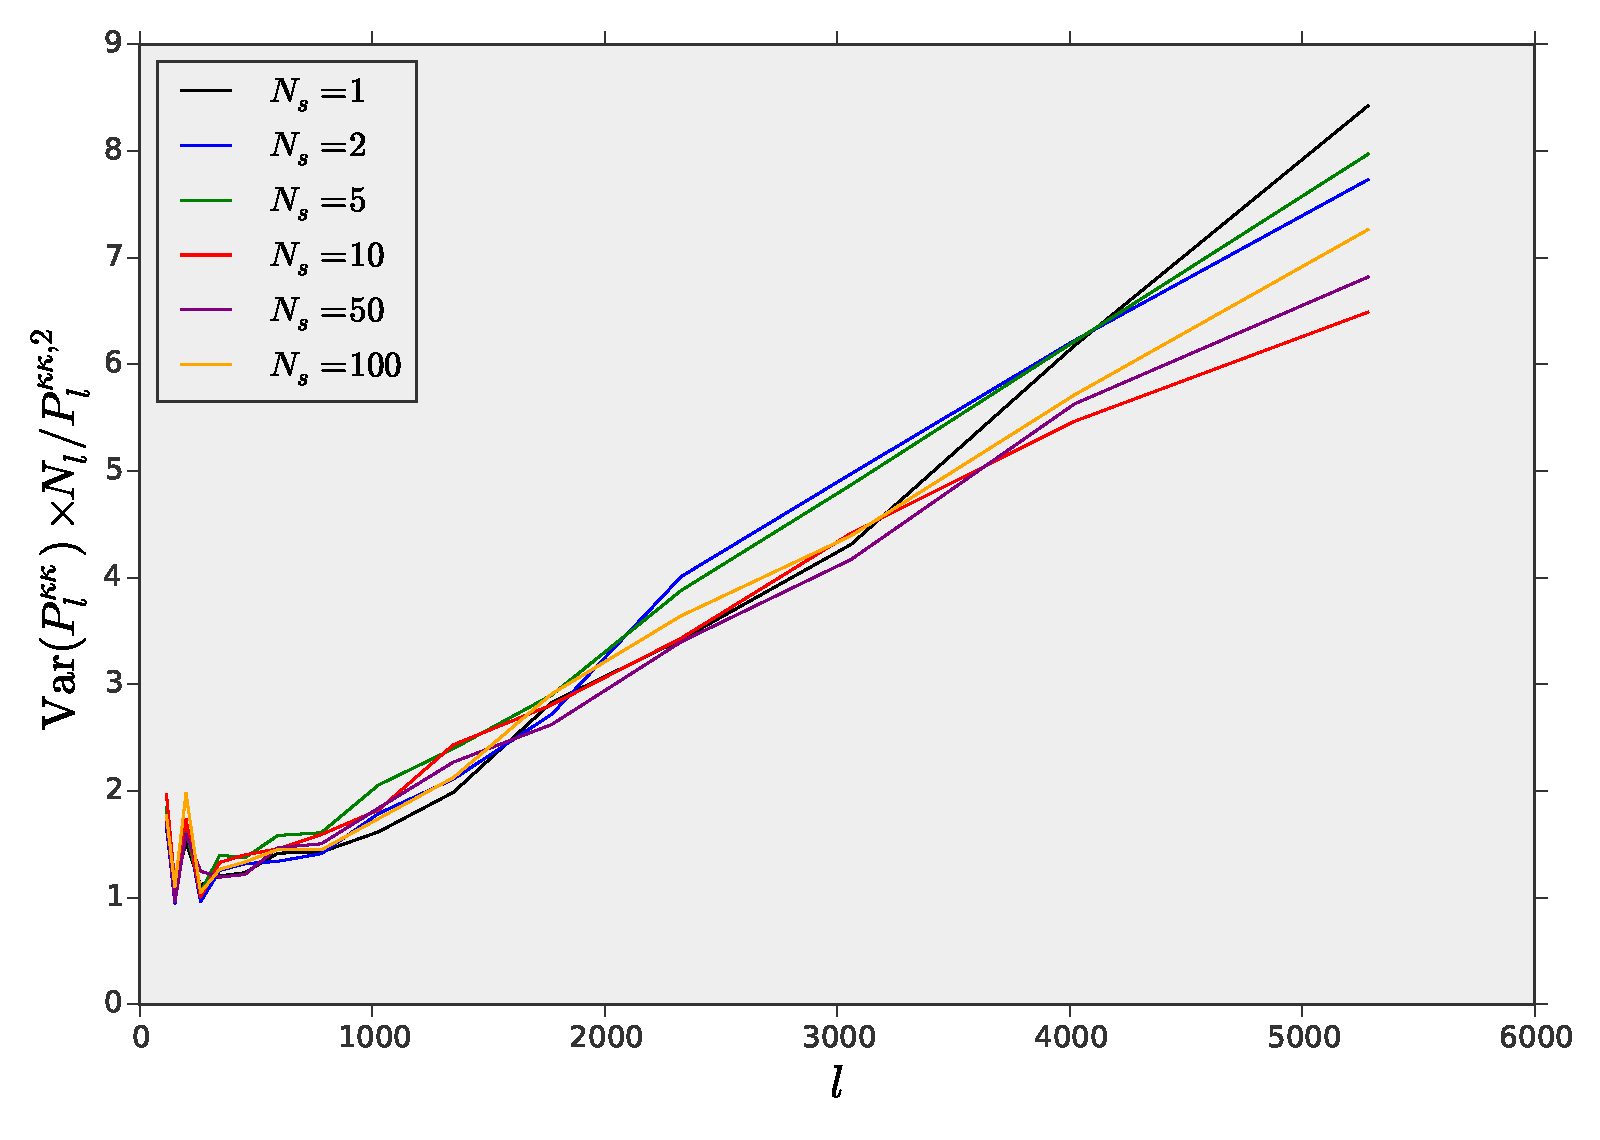
\includegraphics[scale=0.3]{Figures/ps_variance.eps}
\caption{Variance of the $\kappa$ power spectrum as a function of the multipole $l$, in units of the expected gaussian variance from equation (\ref{gaussianvar}). The variance is measured from different shear ensembles with $N_s=$1 (black), 2 (blue), 5 (green), 10 (red), 50 (purple), 100 (orange). }
\label{ps_var}
\end{figure}

\begin{figure}
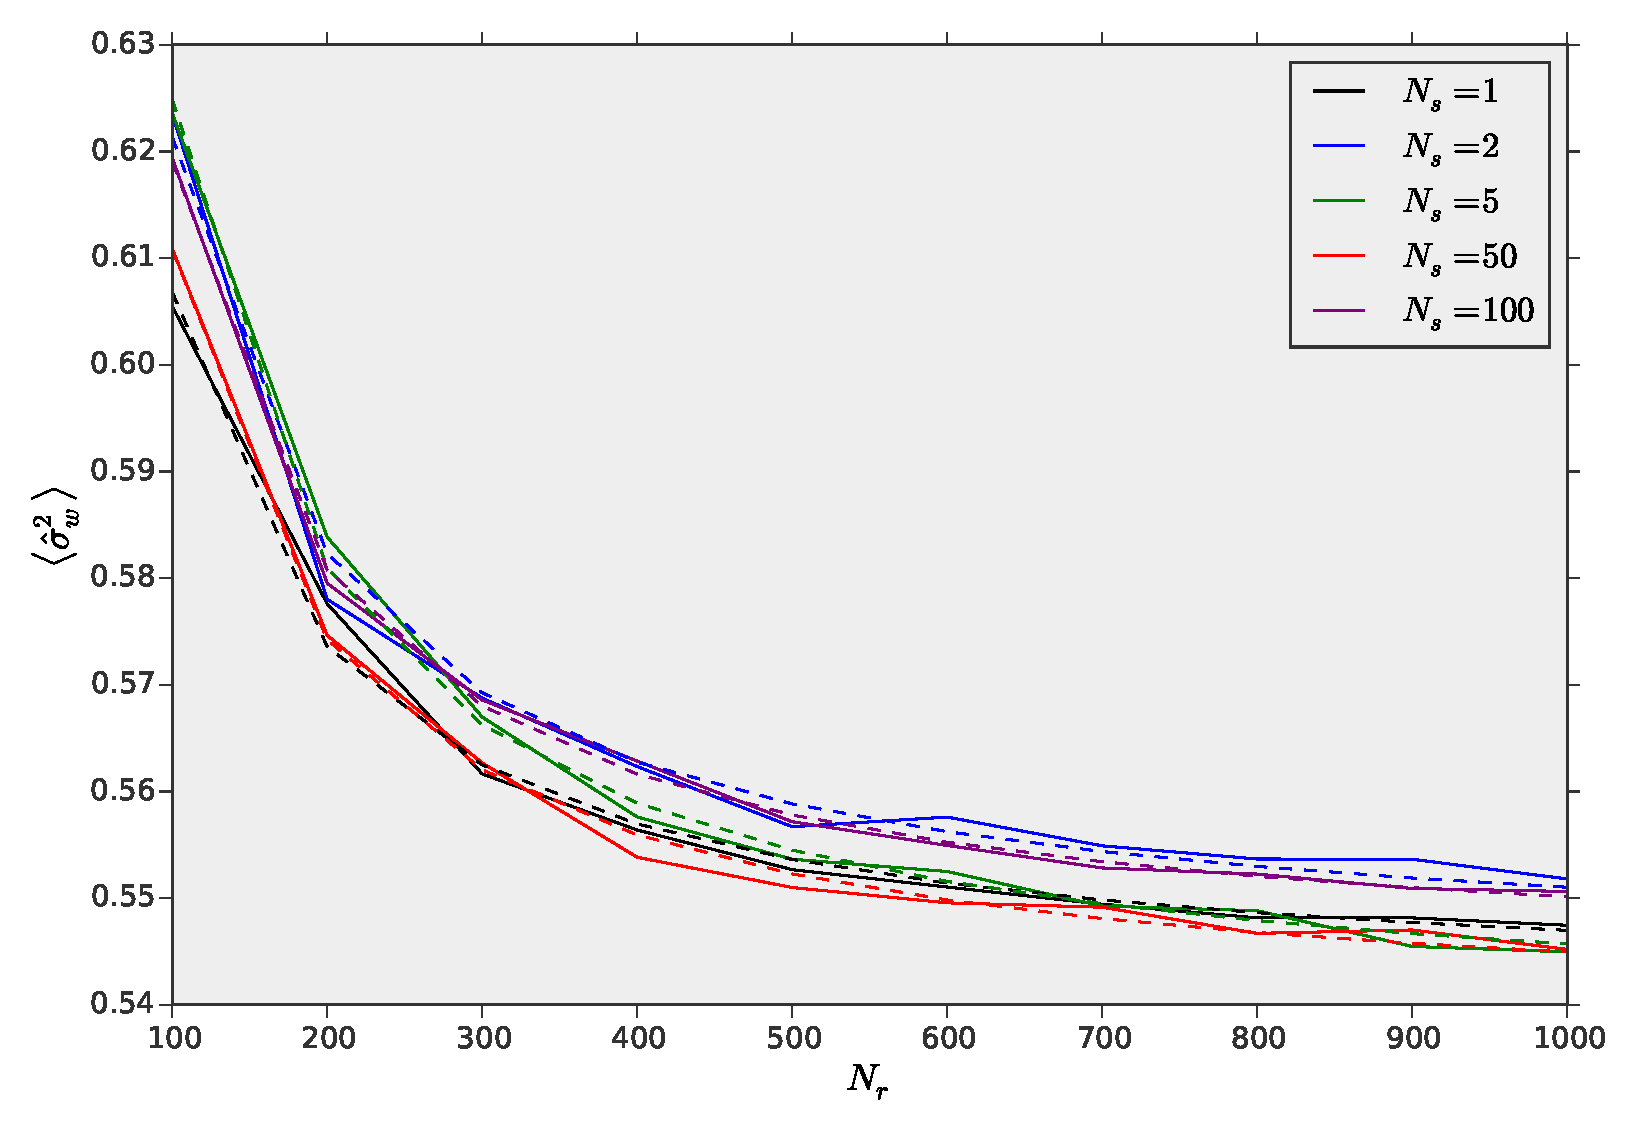
\includegraphics[scale=0.3]{Figures/scaling_nr.eps}
\caption{Expectation value of the variance on $w$, $\langle\h{\sigma}^2_w\rangle$, as a function of the number of mock realizations $N_r$ used in the feature covariance estimator (\ref{covest}). Results for different mock ensembles generated with $N_s=$1 (black), 2 (blue), 5 (green), 50 (red), 100 (purple) are shown. The figure shows both the measured trends (solid lines) and their best fits according to equation (\ref{dodelsonscaling}). }
\label{wvar_nr}
\end{figure}

\begin{table}
\begin{center}
\begin{tabular}{r|rr}
\toprule
 $N_s$ &  $D$(diagonal) &  $D$(full) \\ \hline
\midrule
    1 &   2.8 &  12.3 \\
    2 &   2.1 &  14.4 \\
    5 &   2.6 &  16.4 \\
   10 &   3.1 &  14.6 \\
   20 &   2.4 &  15.8 \\
   30 &   2.5 &  15.4 \\
   40 &   2.7 &  15.7 \\
   50 &   2.5 &  13.6 \\
   60 &   2.7 &  13.3 \\
   70 &   2.4 &  15.0 \\
   80 &   2.4 &  15.6 \\
   90 &   2.6 &  14.1 \\
  100 &   2.2 &  14.1 \\
  150 &   2.3 &  13.9 \\
  200 &   2.6 &  18.2 \\
\bottomrule
\end{tabular}
\end{center}
\caption{Effective dimensionality of the power spectrum feature space $D$ computed fitting the measured $w$ variance with the scaling relation (\ref{dodelsonscaling}). We show both cases in which we consider the full covariance matrix and the case in which we artificially zero out all the off diagonal elements.}
\label{dimtable}
\end{table}

\begin{figure}
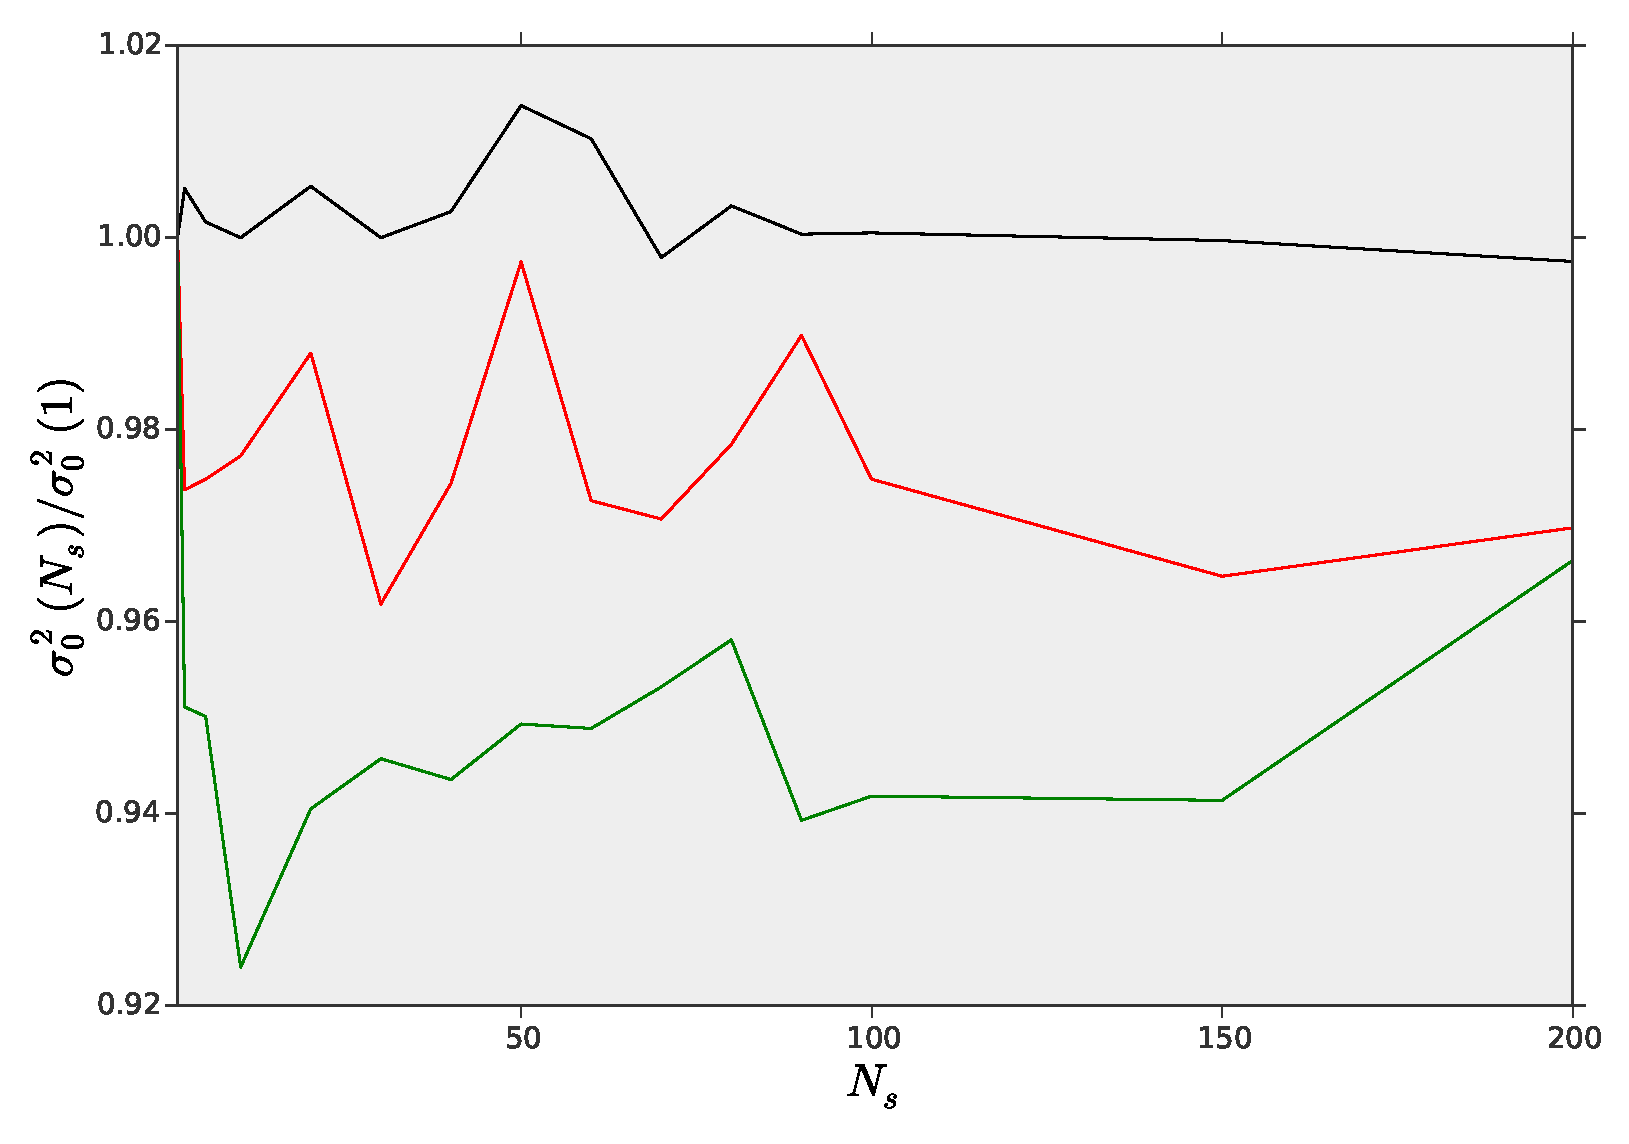
\includegraphics[scale=0.3]{Figures/scaling_ns.eps}
\caption{Expectation value of the variance on $w$, $\langle\h{\sigma}^2_w\rangle$, varying the mock ensemble used to compute the covariance estimator (\ref{covest}). We factored out the $(1+D/N_r)$ dependence, showing only the dependence of $\sigma_0^2$ on $D$. Different choices of $N_r=$100 (black), 300 (blue), 500 (green), 700 (red), 900 (purple) are shown for comparison.}
\label{wvar_ns}
\end{figure}

In this section we outline the main results of this work. We show the qualitative behavior of the $P^{\kappa\kappa}$ probability distribution function (PDF) in ensembles built with different $N_s$. We also show how the forecasts on the Dark Energy equation of state, $w$, depend on $N_s$ and $N_r$. Figure \ref{ps_pdf} shows the power spectrum PDF at four selected multipoles, while Figure \ref{ps_var} shows the variance in each multipole. This result is compared to the one that we would obtain assuming that the convergence is a Gaussian random field
\begin{equation}
\label{gaussianvar}
\mathrm{Var}(P^{\kappa\kappa}(l)) = \frac{P^{\kappa\kappa,2}(l)}{N(l)}
\end{equation}
%
where $N(l)$ is the number of modes used to estimate the power spectrum at $l$, which depends on the mock size $\theta_{box}$ and on the width of the $N_b$ multipole bands. Figure \ref{wvar_nr} and Table \ref{dimtable} show the scaling of the expectation value of $\h{\sigma}_w^2$ with the number of mocks $N_r$ and compare it with the known result obtained in \citep{DodelsonSchneider13}. Figure \ref{wvar_ns} shows the effect of varying $N_s$ on the $w$ constraint. The expectation values $\h{\sigma}^2_w$ (equations (\ref{estimatorcovariance}),(\ref{ourscaling})) have been computed averaging over 100 independent resamples of the $P^{\kappa\kappa}$ ensembles. For the true feature covariance matrix $\langle(\bbh{d}-\bb{d}_0)(\bbh{d}-\bb{d}_0)^T\rangle=\bb{C}$ we use the estimated covariance from the $N_s=200$ ensemble. 


%%%%%%%%%%%%%%%%%% DISCUSSION %%%%%%%%%%%%%%%%%%%%%%%%%%%%%%%%%%%%%

\section{Discussion}

In this section we discuss our main findings. Figure \ref{ps_pdf} shows that, although different choices of $N_s$ do not seem to affect the power spectrum PDF at large scales (top two panels), there are some qualitative differences on small scales (bottom two panels), on which a shear ensemble built with a small $N_s$ might not have the same statistical behavior of ensembles built with large $N_s$. Figure \ref{ps_var} shows the variance of convergence power spectrum computed from different ensembles, in units of the Gaussian expectation. We find that, even with $N_s=1$, our results are in good agreement with the ones obtained by \citep{Sato12}, which used $N_s=400$. This fact by itself is not sufficient to conclude that $N_s$ does not have an effect on parameter inferences, since these depend on the cross band covariances. 

In Figure \ref{wvar_nr} we examine how the $w$ constraint depends on the number of mocks used to estimate the covariance, and we find good agreement with \citep{DodelsonSchneider13}. We determine the effective dimensionality of the feature space, $D$, with a linear regression using equation (\ref{ourscaling}) and we find that this depends strongly on how the noise is distributed across the covariance matrix estimator $\bbh{C}$. In particular we find that when every element in the covariance is subject to noise $D$ is close to the number of bands used $N_b=15$, but when we artificially zero out the off diagonal elements of $\bbh{C}$, the effective dimensionality drops to $D\approx2.5$. Finally, Figure \ref{wvar_ns} shows the dependence of the dark energy constraint with $N_s$ and $D$. We find that, in the range $N_s\in[1,200]$ the $w$ inferred variance has sub--percent fluctuations for both the diagonal and full $\bbh{C}$ cases, while there is a $\sim$10\% change in $\sigma^2_0(N_s,w)$ when the effective dimensionality $D$ is different. Finally, the different lines in Figure \ref{wvar_ns} show that equation (\ref{ourscaling}) is a good model for the variance scaling. 

%%%%%%%%%%%%%%%%%% CONCLUSION %%%%%%%%%%%%%%%%%%%%%%%%%%%%%%%%%%%%%

\section{Conclusion}

In this work we examine the effect of $N$--body simulations based shear ensembles on forecasted cosmological constraints. Our main results can be summarized as follows:

\begin{itemize}
\item The variance scaling relation proposed by \citep{DodelsonSchneider13} is a good approximation regardless of $N_s$
\item The fluctuations in the $w$ forecasted variance due to varying $N_s$ are sub--percent, and this effect is sub--dominant with respect of varying the effective dimensionality of the feature space, which in the end is controlled by how the noise is distributed in the covariance estimator
\end{itemize}
%
Future prospects of this work involve extending this analysis to more general feature spaces, such as the ones that characterize non--Gaussian statistics such as shear peaks and higher moments of $\kappa$ fields. In order to scale these considerations to future surveys such as LSST, it is necessary to see if our findinds hold when challenged by larger and higher resolutions $N$--body simulations.  

%%%%%%%%%%%%%%%%%%%%%%%%%% ACKNOWLEDGMENTS %%%%%%%%%%%%%%%%%%%%%%%%%%%%%%%%%%%%%%%%%%%%%%%%%%%%%%
 

\section*{Acknowledgements}


\bibliography{ref}
\label{lastpage}
\end{document}
